\documentclass[../../relatorio.tex]{subfiles}

\begin{document}

\subsection{Dívida Pública}

\begin{figure}[ht]
  \begin{minipage}{0.70\textheight}
    \centering
      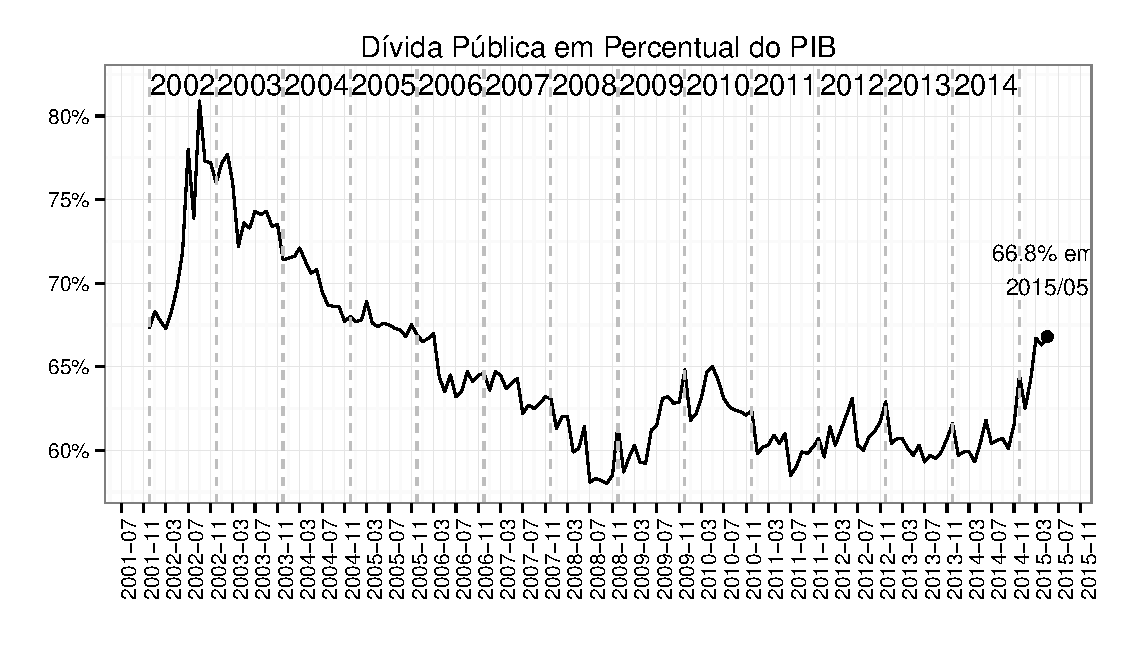
\includegraphics[width=17cm]{DividaPublica.pdf}
  \end{minipage}
\end{figure}

A \textbf{dívida pública} abrange empréstimos contraídos pelo Estado junto a instituições financeiras públicas ou privadas, no mercado financeiro interno ou externo, bem como junto a empresas, organismos nacionais e internacionais, pessoas ou outros governos.

A dívida pública federal pode ser formalizada por meio de contratos celebrados entre as partes, ou por meio da oferta de títulos públicos emitidos pelo Tesouro Nacional.


Teoricamente, a dívida pública é classificada como dívida interna ou dívida externa, de acordo com a localização dos seus credores e com a moeda envolvida nas operações.

Historicamente, é muito importante estudar a evolução dessas duas dívidas de forma separada. Porém, atualmente, diante da ausência de restrições ao ingresso e saída de moedas internacionais no Brasil por meio do sistema bancário – o que convencionalmente se chama de liberdade de movimentação de capitais – esses conceitos precisam ser revistos, pois bancos e instituições estrangeiras são credores da dívida “interna”, da mesma forma que bancos e instituições brasileiros podem ser credores da dívida “externa”. Além disso, o Brasil tem emitido títulos da dívida externa em reais. Tais exemplos demonstram que, atualmente, a natureza de ambas as dívidas – interna e externa – se confunde. Somando a chamada dívida “interna” com a “externa”, temos o total da dívida pública brasileira. \footnote{http://www.auditoriacidada.org.br/}

\pagebreak
\end{document}
